%%%%%%%%%%%%%%%%%%%%%%%%%%%%%%%%%%%%%%%%%
% Science Publications
% LaTeX Template
% Version 1 (1/5/2023)
%
% Original author: Shubhi Parth Manan
% Ali Asfour (ali.f.asfour@gmail.com)
%
%%%%%%%%%%%%%%%%%%%%%%%%%%%%%%%%%%%%%%%%%

%----------------------------------------------------------------------------------------
%	PACKAGES AND OTHER DOCUMENT CONFIGURATIONS
%----------------------------------------------------------------------------------------
\documentclass[fleqn,10pt]{thescipub} % Document font size and equations flushed left
%\usepackage{fontspec}
%\fontspec[WordSpace=0.5]{Times New Roman}
\usepackage{natbib} 
\usepackage[english]{babel} % Specify a different language here - english by default
%----------------------------------------------------------------------------------------
%	Justification align and remove hyphenation
%----------------------------------------------------------------------------------------
\tolerance=1
\emergencystretch=\maxdimen
\hyphenpenalty=10000
\hbadness=10000
\usepackage{indentfirst}
\setlength{\parindent}{0.5cm}
%----------------------------------------------------------------------------------------
%	COLUMNS
%----------------------------------------------------------------------------------------

\setlength{\columnsep}{0.76cm} % Distance between the two columns of text
\setlength{\fboxrule}{0.75pt} % Width of the border around the abstract

%----------------------------------------------------------------------------------------
%	COLORS
%----------------------------------------------------------------------------------------

\definecolor{color3}{RGB}{25,72,126} % Color of the boxes behind the abstract and headings

%----------------------------------------------------------------------------------------
%	HYPERLINKS
%----------------------------------------------------------------------------------------

\usepackage{hyperref} % Required for hyperlinks
\hypersetup{hidelinks,colorlinks,breaklinks=true,urlcolor=black,citecolor=black,linkcolor=black,bookmarksopen=false,pdftitle={P-BOT: A Personal PDF Chatbot},pdfauthor={Author}}

%----------------------------------------------------------------------------------------
%	ARTICLE INFORMATION
%----------------------------------------------------------------------------------------
\JournalInfo{Journal Of Computer Science} % Journal information

\PaperTitle{P-BOT: A Personal PDF Chatbot} 
\Authors{Parth Shah\textsuperscript{1}, Abhijit Patil\textsuperscript{1}, Shubhi Parashar\textsuperscript{1}, Manan Salia\textsuperscript{1}} % Authors
\affiliation{\textsuperscript{1}\textit{Department of Computer Engineeering, K J Somaiya Institute of Technology, Mumbai, India;}} % Author affiliation
%\affiliation{\textsuperscript{2}\textit{Department of Computer Engineeering, NK J Somaiya Institute of Technology, Mumbai, India;}} % Author affiliation
%\affiliation{\textsuperscript{3}\textit{Department of Computer Engineeering, NK J Somaiya Institute of Technology, Mumbai, India;}} % Author affiliation
%\affiliation{\textsuperscript{4}\textit{Department of Computer Engineeering, NK J Somaiya Institute of Technology, Mumbai, India;}} % Author affiliation


\Keywords{Chatbot, PDF, GPT, LLM, Infromation Retrieval, P-BOT.} % Keywords - if you don't want any simply remove all the text between the curly brackets
\newcommand{\keywordname}{Keywords} % Defines the keywords heading name

%----------------------------------------------------------------------------------------
%	ABSTRACT
%----------------------------------------------------------------------------------------

\Abstract{In an age where PDFs store vast amounts of information, the labor-intensive process of manually sifting through complex documents presents a significant hurdle in academic research and knowledge management. P-BOT, the Personalized PDF Chat Bot, offers an ingenious solution by leveraging advanced ’Machine Learning’ (ML) and ’Natural Language Processing’ (NLP) techniques. It not only parses individual PDFs but can also handle multiple PDFs as input, creating structured knowledge bases for each. P-BOT’s user-friendly chat interface allows users to ask plain language questions and receive precise answers directly from the PDF content, revolutionizing PDF interaction. This innovative fusion of NLP and ML technologies enhances academic research and knowledge utilization, empowering researchers to efficiently extract insights from multiple PDFs and simplifying the journey from information acquisition to knowledge application.}

%----------------------------------------------------------------------------------------

\begin{document}
\captionsetup[figure]{labelfont={bf},name={Fig.},labelsep=period}
\captionsetup[table]{labelfont={bf},name={Table},labelsep=period}
\flushbottom % Makes all text pages the same height

\maketitle % Print the title and abstract box

%----------------------------------------------------------------------------------------
%	ARTICLE CONTENTS
%----------------------------------------------------------------------------------------

\section*{Introduction} The advent of 'Artificial Intelligence Generated Content '(AIGC) (J. Wu et al., 2023; Wang, Y. et al., 2023 ; Wu, T. et al., 2023) has unfolded as a prominent response to the challenges posed by digital intelligence in the modern digital economy. AIGC harnesses the power of artificial intelligence to streamline or even replace manual content creation processes, producing content that aligns with user-provided keywords and specifications. The ongoing progress in extensive model algorithms has significantly strengthened the capabilities of AIGC, establishing it as a promising tool that enhances convenience in various aspects of our daily activities. Positioned as a pioneering technology, AIGC holds boundless potential to support a wide array of downstream applications. The realm of content creation and knowledge representation is undergoing a pivotal transformation, largely driven by the widespread adoption of substantial artificial intelligence models like ChatGPT(Wang, Y. et al., 2023).  AIGC, driven by these generative large AI algorithms, is at the forefront of this paradigm shift. It empowers users by aiding or even substituting human efforts in generating extensive, top-tier, and remarkably human-like content swiftly and cost-effectively, all hinging on user-provided prompts. 

\parskip=0.5\baselineskip

Generative AI(Gozalo-Brizuela et al., 2023), a crucial element within the 'Artificial Intelligence Generated Content' (AIGC) ecosystem, plays a crucial role in influencing the course of AI-powered interactions. It plays a significant part in empowering the development of conversational agents and chatbots capable of engaging in dynamic, contextually relevant conversations, thereby enriching user experiences across a wide spectrum of applications, ranging from customer service to content creation. This forward-thinking technology continues its evolution, continuously expanding the horizons of what AI can accomplish in terms of comprehending and producing human language, ultimately paving the way for more intelligent and responsive AI systems.

Leveraging Generative AI represents a strategic advantage, as it enables the integration of advanced tools capable of addressing inquiries pertaining to PDF documents. In the contemporary digital era, libraries have evolved beyond their traditional physical confines to encompass a vast array of online resources tailored to serve their patrons. A widely adopted format for these digital resources is the Portable Document Format (PDF), which facilitates the seamless dissemination of information while preserving the original document's layout and formatting. Consequently, PDFs have gained popularity, particularly for the storage and distribution of academic articles and research reports. Nevertheless, PDFs present a unique challenge within library systems, primarily stemming from their limited interactivity when compared to dynamic web pages and other digital content sources. Unlike more interactive resources, PDFs lack essential features that enable users to conduct in-document searches, annotate text, or navigate through different sections seamlessly. This deficiency can result in user frustration and disengagement, particularly when users seek more interactive functionalities. Consequently, addressing the issue of PDF interaction within library systems emerges as a pivotal endeavor. The enhancement of user engagement and satisfaction relies on the provision of more interactive PDF experiences. Libraries can significantly elevate the user experience by offering interactive PDFs, thereby fostering a greater likelihood of users returning to the library as a valuable and user-centric resource.

A promising solution to the aforementioned challenge is the introduction of the P-BOT, an acronym denoting the "Personalized PDF Chat-BOT." The P-BOT represents an innovative online software platform that leverages the formidable capabilities of the ChatGPT API, offering users a more intuitive and seamless method for engaging with PDF documents. Through seamless integration of the P-BOT into library systems, patrons gain access to a chat-based interface that enables efficient and natural interactions with digital resources, including books, research papers, theses, manuals, essays, and a diverse range of academic content. P-BOT empowers users to pose queries, request assistance, and effortlessly navigate through PDF documents, thus serving as a valuable and transformative addition to library systems. This cutting-edge tool not only enhances user experiences but also streamlines the accessibility and usability of library resources, aligning perfectly with the evolving needs of modern library patrons, researchers, and scholars, thereby contributing to the advancement of knowledge dissemination. P-BOT will incorporate the feature of uploading multiple PDFs, including PDFs of substantial length, such as those spanning up to 1,000 pages.

\section{Literature Survey}

\subsection{History of Text Extraction}

In the late 1990s, as the usage of PDF documents surged, initial efforts were made to extract text from these files. These early text extraction techniques primarily focused on dissecting the PDF structure to identify and retrieve text content. However, they encountered limitations, particularly in terms of accuracy and their ability to preserve document formatting. 

To address these challenges, Optical Character Recognition (OCR) technology was introduced(Mori, Shunji et al., 1992), aiming to convert printed and handwritten text into digital format. OCR's primary objective was to facilitate the transition from paper-based content to the digital realm, enhancing accessibility, editability, and searchability. It not only automated data entry, reducing errors and costs, but also streamlined information retrieval from scanned documents and archives. OCR played a pivotal role in extracting text from tangible documents, images, and PDFs, making content searchable, editable, and available for diverse applications. Moreover, it significantly improved text accessibility for individuals with visual impairments by converting text into a readable format for assistive technologies. The introduction of OCR marked a groundbreaking transformation in how text-based information is managed, bridging the analog and digital realms.

Tesseract OCR(Smith, Ray, 2007), an open-source Optical Character Recognition engine developed by Google, is renowned for its exceptional precision in identifying printed text within scanned documents, images, and PDFs. Tesseract is compatible with various languages, capable of extracting text from diverse fonts and text sizes. Its adaptability and ongoing enhancements have solidified its status as a favored solution for automating data entry, digitizing printed resources, enabling text searches within images, and supporting a variety of applications that require the transformation of visual text into machine-readable text.

While traditional OCR technology excelled within predefined formats and fonts, machine learning (ML) and deep learning (DL) have unfolded as superior alternatives due to their adaptability, superior accuracy, and contextual comprehension of text. These models surpass the rigid constraints of OCR, accommodating a wide range of document layouts, languages, and even handwritten content. Their versatility enables the precise extraction of text, making them suitable for handling complex documents. Moreover, these models continuously improve their performance through fine-tuning with new data, ensuring their ongoing relevance and effectiveness in an ever-evolving digital landscape.

The utilization of machine learning and deep learning methods, including natural language processing (NLP) models, has led to significant advancements in text extraction from PDFs. These advanced models excel at identifying and extracting text content from intricate PDF documents, including those with multiple columns, tables, and a wide variety of fonts, further enhancing the efficiency and accuracy of text extraction processes.

\subsection{History of Text Generation}

Understanding the landscape of generative AI models is crucial for making informed choices regarding their suitability for various applications within our software platform. The foundations of generative models trace back to the 1950s when pioneering efforts led to the development of "Hidden Markov Models" (HMMs)(L. Rabiner, B. Juang, 1986; M. I. Mohd Yusoff et al., 2014) and "Gaussian Mixture Models" (GMMs)(Viroli et al., 2017). These early models exhibited the capability to generate sequential data, a milestone achievement with notable applications in speech recognition and time series analysis. However, it was not until the rise of deep learning in more recent years that generative models truly began to shine. Deep learning models, including neural networks, "Recurrent Neural Networks" (RNNs), and "Convolutional Neural Networks" (CNNs), have been instrumental in significantly enhancing the performance and versatility of generative AI. The field has been transformed by their capacity to grasp intricate patterns, encompass enduring relationships, and produce data in high dimensions.

\subsubsection{Language Models}

In the realm of natural language processing, statistical language models play a vital role by deducing the probability distribution of natural language.These models are dedicated to estimating the probability of generating a given sentence or predicting the content of the next part of a sentence, which is essential for various downstream NLP tasks. Various modeling methods have been developed to address this, reflecting the technical advancements in the field. Early n-gram language models rely on frequency statistics of n-grams, but they have limitations in handling larger context and symbol combinations. Neural language models (NLM) introduced more complex structures, such as multilayer perceptrons, CNNs and RNNs, improving the representation of words and their context-aware dynamic nature through low-dimensional embeddings.



Among the earliest methods for sentence generation, N-gram language modeling(Pauls et al., 2011; Niesler et al., 1996;  Bickel, S. et al., 2005) stands as a foundational approach in the world of Natural Language Processing (NLP). N-grams represent contiguous sequences of words, symbols, or tokens in textual or speech data, defined as neighboring sequences within a given document. These N-grams are integral to a wide array of applications in NLP, extending their influence to domains such as statistical natural language processing, speech recognition, phonemes, machine translation, predictive text input, and more, where the modeling inputs rely on N-gram distributions. N-grams themselves manifest as co-occurring words or items within a specific window, advanced by a fixed number of words or tokens, often referred to as "k." These co-occurring words are termed "n-grams," with "n" signifying the length of the word string considered in constructing these n-grams. The spectrum encompasses unigrams (single words), bigrams (two-word sequences), trigrams (three-word sequences), 4-grams, 5-grams, and so forth. N-grams are harnessed extensively in NLP, text mining, and various natural language processing tasks. Language model development in NLP, for instance, leverages not just unigram models but extends to bigram and trigram models. Major tech companies, including Google and Microsoft, have ventured into constructing expansive web-scale n-gram models, which find utility in NLP tasks like spelling correction, word segmentation, and text summarization. Furthermore, N-grams are vital in crafting features for supervised Machine Learning models, such as "Support Vector Machines" (SVMs), "Maximum Entropy" (MaxEnt) models, and "Naive Bayes classifiers". The fundamental concept lies in enriching the feature space with tokens like bigrams, trigrams, and more advanced n-grams, transcending the limitations of relying solely on unigrams.




The utilization of N-gram language modeling has indeed played a pivotal role in advancing the domain of text generation. However, it is essential to recognize that its effectiveness encounters constraints, particularly when dealing with longer and more intricate sentences. These limitations have acted as a catalyst for the emergence of "Recurrent Neural Networks" (RNNs), which represent a groundbreaking development in the realm of language modeling tasks. In their initial iterations, RNNs brought forth a crucial innovation by granting the ability to model longer dependencies within textual data. This innovation opened doors to the generation of more extensive and intricate sentences, marking a significant leap in the quest for improved text generation techniques.



In the broader context of natural language processing (NLP), it's important to note that the narrative of innovation did not begin with RNNs alone. Convolutional Neural Networks (CNNs)(Yin, Wenpeng, et al., 2017) had already made substantial contributions to the field before the advent of RNNs. These two deep neural network (DNN) architectures, CNNs and RNNs, have become foundational tools in NLP tasks. CNNs, in particular, excel in capturing position-invariant features, making them adept at identifying local patterns, n-grams, and various features within textual data. Their versatility has been evident across an array of NLP tasks, encompassing text classification, semantic similarity analysis, document classification, question answering, named entity recognition and text generation. Nonetheless, it's essential to acknowledge that while CNNs offer compelling advantages, they may not be universally suitable for all NLP applications. This consideration arises from the inherent design of CNNs, which is not primarily tailored for sequential data processing. In the domain of NLP, textual data inherently comprises sequences of words or tokens, presenting a unique challenge when employing CNNs for efficient data processing.


On the contrary, RNNs are a specialized class of neural networks explicitly engineered to handle sequential data. In a standard Recurrent Neural Network, each output depends on both the current input and the internal memory or hidden state inherited from the previous step. This intrinsic mechanism empowers RNNs to retain vital information about past inputs, enabling them to effectively capture intricate sequential relationships in data. 




In 1997, the introduction of "Long Short-Term Memory" networks, abbreviated as LSTMs(Hochreiter et al., 1997), marked an important breakthrough in the field of recurrent neural networks (RNNs). LSTMs were specifically engineered to address the formidable challenge of the vanishing gradient problem, a recurring issue that often hinders the training of deep neural networks, especially within the context of RNNs and specific deep feedforward networks. The vanishing gradient problem arises when the gradients of the loss function concerning the network's parameters diminish to near-zero levels as they traverse backward through the network's layers during the training phase.


LSTMs excel in capturing long-term dependencies within sequences, offering a solution to issues related to backflow errors and the need to minimize time intervals. Unlike earlier methods, LSTMs swiftly learn to discern multiple occurrences of a specific element in an input sequence, even when those occurrences are widely spaced, without relying on specific short-time-lag training examples. These networks demonstrate the remarkable ability to effectively capture and connect information across substantial time intervals, surpassing 1000 discrete-time steps. This capability is achieved by maintaining a consistent flow of error information through dedicated units referred to as "constant error carousels." Additionally, LSTMs employ multiplicative gate units that learn to regulate access to this constant error flow, determining when to open or close it.

However, it's crucial to acknowledge that LSTMs are not without their challenges. They are notably challenging to train due to their involvement in very long gradient paths(Hochreiter et al., 1998). LSTMs are susceptible to overfitting, especially when dealing with limited datasets. Effective performance often necessitates a substantial amount of training data, and they may struggle to generalize effectively when data is scarce. Furthermore, LSTMs can be memory-intensive, particularly when dealing with extended sequences or complex model architectures. Another notable aspect is that LSTMs are frequently regarded as inscrutable models, which can pose challenges in understanding the decision-making processes underlying their predictions. This opacity becomes a significant concern in contexts where transparency and interpretability hold paramount importance.



In the quest to generate sentences possessing similar attributes through Long Short-Term Memory networks (LSTMs), a novel strategy known as Syntactic and Semantic LSTM (SSLSTM)(Liang et al., 2021) was introduced. The SSLSTM method capitalizes on the combined syntactic and semantic cues embedded within sentences to evaluate their resemblance. At the core of SSLSTM is its sentence model, a pivotal element that utilizes both sentence-level syntactic structures and word-level semantic information to aptly encapsulate the fundamental linguistic qualities of input sentences.


The process begins with the segmentation of text into individual words, employing word embeddings to encode these words with contextual information. CoreNLP, a natural language processing toolkit, is subsequently employed to generate related sentences by extracting syntactic word relationships, thereby adding a layer of syntactic understanding to the similarity measurement. Additionally, an offline package of WordNet 3(Miller, George A., 1995) comes into play, serving the purpose of identifying analogous nouns within sentences and simplifying their overall complexity. This comprehensive approach amalgamates the advantages of both syntactic and semantic analyses, providing a sturdy technique for assessing and creating sentences that possess common linguistic characteristics. It represents a notable advancement in this field, pushing the boundaries of what is achievable in the domain.



Introduced in 2014, Generative Adversarial Networks (GANs)(Wang, Kunfeng, et al., 2017) have emerged as a prominent class of machine learning models, constituting a fascinating interplay between two neural networks: the generator and the discriminator. This dynamic training process, as outlined in "Generative Adversarial Networks: Introduction and Outlook," is fundamentally competitive in nature. The generator's role is to create synthetic data, while the discriminator's objective is to distinguish between real data and the generated counterparts. It is through this adversarial back-and-forth that GANs master the art of producing high-quality data that is virtually indistinguishable from authentic data.


GANs have made significant strides in various domains, including image synthesis, data augmentation, style transfer, and text generation, thus catalyzing advancements in generative modeling and fostering creative applications in the realm of artificial intelligence. Despite their notable achievements, GANs are not without their limitations. Successful operation of GANs hinges on the intricate balance and synchronization between their two adversarial networks during training, a task that can often introduce challenges related to training instability. Furthermore, GANs share the common issue of poor interpretability with other neural network-based generative models. In addition, they can encounter the challenge of "mode collapse," a situation in which the generated images tend to exhibit similar color or texture themes, thereby restricting the diversity of their output. These nuanced aspects of GANs underscore the ongoing research efforts aimed at addressing their challenges while maximizing their creative potential.


The Gated Recurrent Unit (GRU)(Tang, Xianlun, et al., 2019) stands as a notable player in the domain of Recurrent Neural Networks (RNNs), also introduced in 2014, demonstrating remarkable prowess in Natural Language Processing. GRUs, akin to other RNNs, are meticulously designed for the processing of sequential data, rendering them exceptionally well-suited for tasks within the realms of NLP and time-series analysis. These networks incorporate a gating mechanism, similar to the Long Short-Term Memory (LSTM) networks, albeit with a relatively simpler architectural structure.


The inception of the GRU marked an important development, with the introduction of reset and update gates that enable the capture of dependencies across varying time scales. In contrast to LSTMs, GRUs exhibit a more direct exposure of their hidden state and forgo the use of an output gate for control. This streamlined architectural design has the distinct advantage of reducing the number of parameters within the GRU, which, in turn, contributes to a more straightforward convergence during the training process. Both LSTM and GRU have found extensive applications in text classification tasks, underscoring their collective significance in NLP.


However, it is important to recognize that GRUs, unlike LSTMs, lack dedicated memory cells, rendering them somewhat less adept at tasks that demand meticulous memory management. Moreover, their reduced set of gating mechanisms, relative to LSTMs, may somewhat limit their ability to finely control the flow of information. 

In response to these challenges and the limitations associated with Convolutional Neural Networks (CNNs) and traditional RNNs, the Transformer model emerged as a transformative solution, ushering in a new era in natural language processing and addressing a wide range of tasks with remarkable efficiency and effectiveness.

The Transformer model has brought about a significant transformation in the world of NLP, ushering in a novel paradigm that unlocks a wide array of potential and opportunities (Vaswani, Ashish, et al., 2017). In stark departure from conventional recurrent connections, the Transformer hinges on two fundamental components: the self-attention mechanism and feedforward neural networks. This architectural choice not only ushers in superior parallelization but also dramatically reduces the training time, setting a new standard for efficiency in NLP.


The core of the Transformer's innovation centers on the self-attention mechanism. This feature empowers the model to evaluate the importance of every word or token within a specific sequence in relation to all the others. Consequently, it enables a holistic comprehension of context and connections across different spans. It accomplishes this by generating attention scores, which gauge the similarity between each pair of tokens and, subsequently, utilizes these scores to blend information from disparate parts of the sequence. The outcome is the creation of context-aware representations for each token, a critical element in the model's success.

The Transformer architecture, as illustrated in Figure 1, is defined by the stacking of numerous layers of self-attention and feedforward neural networks. Every layer operates autonomously, utilizing the self-attention mechanism concurrently across the entire input sequence.This global approach to information capture is followed by the application of feedforward neural networks that further refine and transform the representations.


To ensure the robustness of the model and its ability to learn intricate patterns, various techniques are integrated, such as residual connections and layer normalization. These methods help mitigate the vanishing gradient problem, thus accelerating the training process. Furthermore, Transformers often incorporate positional encodings to provide information about the order or location of tokens in the sequence, as self-attention, while powerful, does not inherently account for positional relationships.
Training the Transformer entails the minimization of a loss function, typically leveraging labeled data and employing backpropagation in conjunction with optimization algorithms like Adam. Once adequately trained, the Transformer stands ready for a myriad of applications, spanning machine translation, text summarization, sentiment analysis, and more. It operates both in an encoder-decoder configuration for sequence-to-sequence tasks and as a standalone model for various tasks, including text classification and language modeling, solidifying its status as a cornerstone in contemporary NLP.

\begin{figure}[htp]
    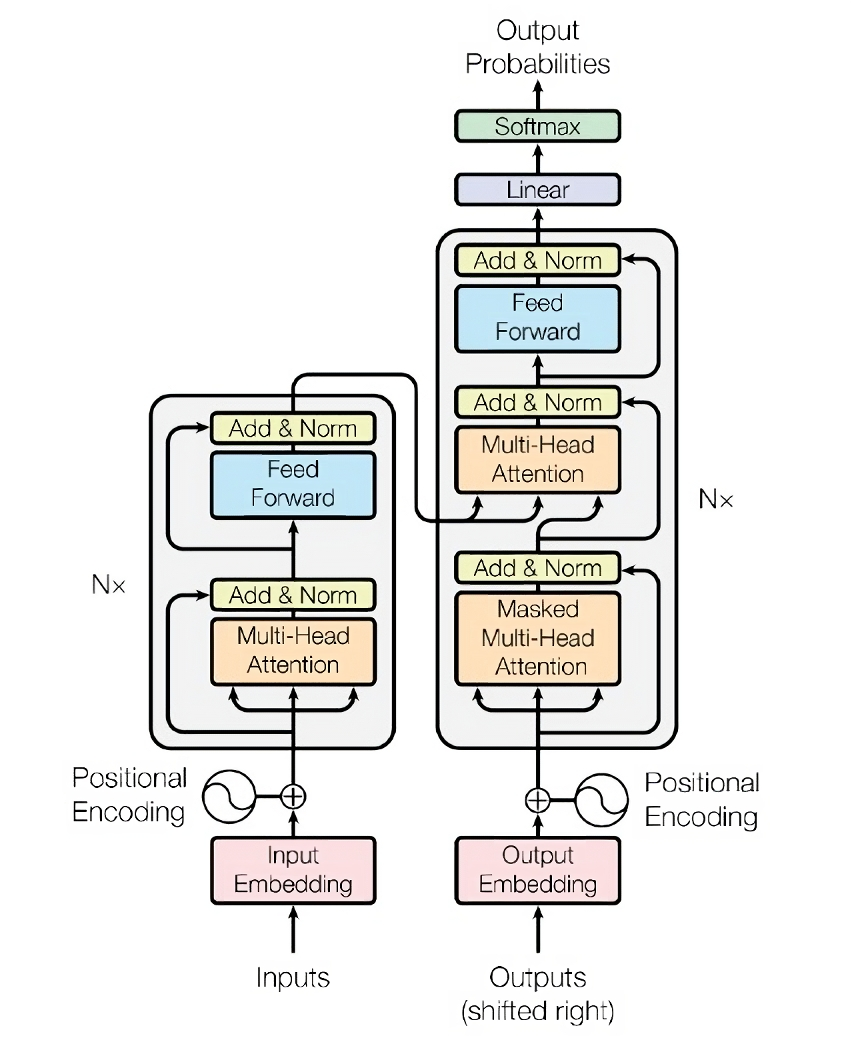
\includegraphics[width=9cm]{transformer}
    \caption{The Transformer model architecture reference Ashish Vaswani et al., 2017}
    \label{fig:galaxy}
\end{figure}



Since 2018, pre-trained language models (PLMs) have garnered significant attention, especially those developed through self-supervised learning on extensive text data. Prominent models such as ELMo, BERT, and GPT-3 have showcased remarkable capabilities across various NLP tasks. PLMs provide adaptable context-aware representations and offer a unified framework for NLP assignments. They exhibit three primary model structures: autoregressive language models (LM), autoencoding LM, and hybrid LM (as depicted in Figure 2) exemplified by GPT, BERT, and T5, respectively. Autoregressive LM primarily focuses on predicting words token by token, whereas autoencoding LM involves masking words within sentences, utilizing bidirectional encoding, and predicting masked words based on contextual cues. Hybrid LM combines these strategies. BERT's outstanding performance has led to its widespread adoption in both academic and industrial settings within the NLP domain.

Leveraging the Transformer architecture, OpenAI has developed a series of GPT models, including GPT-1, GPT-2, GPT-3, and GPT-4. All of these models have demonstrated improvements in language understanding and generation, with GPT-3 being particularly noteworthy for its excellence in text generation tasks and support for zero-shot and few-shot learning scenarios. OpenAI has further advanced large-scale language models with models like GPT-3.5 series, which includes Code-davinci and Text-davinci models. These models have enabled users to leverage advanced language capabilities through APIs and playgrounds. GPT-4, the latest milestone, is a large multimodal model, showing enhanced capabilities in understanding nuanced instructions.

The progress in artificial intelligence has underscored the effectiveness of large models in acquiring intricate features and patterns from raw data. This, in turn, enhances their capacity for comprehending and generating data. Large-scale pre-trained language models, such as those seen in GPT-3 and subsequent versions, demonstrate superior generalization and proficiency in handling various tasks. The adoption of the autoregressive language modeling approach, as seen in GPT-3 and its successors, proves advantageous by directly leveraging natural language to articulate diverse tasks across different domains. Researchers are now keen to investigate the capabilities and transparency of GPT-4, anticipating its contribution to the continuous evolution of artificial intelligence. These advancements underscore the pivotal role that language models play in advancing modern Natural Language Processing (NLP) and AI technologies.

\begin{figure*}
    \centering
    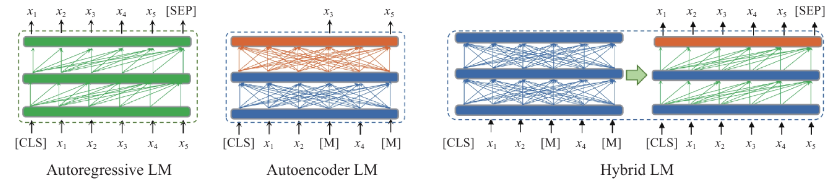
\includegraphics[width=\textwidth]{LMTYPES}
    \caption{Three primary types of PLM: Autoregressive Language Model (LM), Autoencoder Language Model, and Hybrid Language Model. Their operational mechanisms are outlined and compared in the table provided below from Tianyu Wu et al., 2023}
    \label{fig:your_image_label}
\end{figure*}

\begin{table*}
    \centering
    \caption{Comparison of Pre-trained Language Models}
    \begin{tabular}{|p{2cm}|p{3cm}|p{3cm}|p{2cm}|p{2cm}|p{2 cm}|}
        \hline
\center
        \textbf{Aspect} & \textbf{Encoding/Decoding Strategy} & \textbf{Input-Output Example} & \textbf{Learning Paradigm} & \textbf{Support Tasks} & \textbf{Representative Model} \\
        \hline
\center
        Autoregressive LM & Autoregressive models create text in a sequential manner, forecasting each token individually by considering the preceding tokens. & Input text is encoded step by step, generating output sequentially. & Unidirectional prediction from left to right or vice versa. & Language modeling, text generation, and sequence completion tasks. & GPT-3 (Generative Pre-trained Transformer 3) \\
        \hline
\center
        Autoencoder LM & Autoencoder models transform input text into a constant-size representation and subsequently reverse this process to reconstruct the original text. & Input text is compressed into a latent representation and reconstructed during decoding. & Bidirectional encoding and decoding for representation learning. & Data compression, text denoising, and anomaly detection tasks. & BERT (Bidirectional Encoder Representations from Transformers) \\
        \hline
\center
        Hybrid LM & Hybrid models combine elements of both autoregressive and autoencoder LMs to leverage their strengths. & Input text can be processed both sequentially and with bidirectional encoding-decoding. & Combines unidirectional and bidirectional learning strategies. & Adaptable for an extensive array of applications, spanning from text classification and language modeling to text generation. & T5 (Text-to-Text Transfer Transformer) \\
        \hline
    \end{tabular}
\end{table*} 

In 2018, ELMo, which stands for "Embeddings from Language Models," was introduced(Sarzynska-Wawer, Justyna, et al., 2021). It presents a unique way of creating word embeddings, offering distinct representations for each token in a sentence by considering the entire input sentence. These representations are crafted through the utilization of a bidirectional Long Short-Term Memory (LSTM) network, which is trained with a connected language model objective on an extensive text corpus. What distinguishes ELMo is its depth, as it encompasses information from all the internal layers of the bidirectional LSTM. By merging these internal states, ELMo provides comprehensive word representations that capture the intricate and context-specific facets of word meaning and syntax. Notably, ELMo representations have displayed substantial improvements in performance across a spectrum of language comprehension tasks, including applications like textual entailment, question answering, and sentiment analysis.
ELMo is a model that enhances the performance of various natural language processing (NLP) tasks. It builds upon the Bidirectional Attention Flow model (BiDAF) by introducing several improvements, including the incorporation of a self-attention layer, simplification of pooling operations, and the substitution of LSTMs with gated recurrent units (GRUs). When ELMo is integrated into the baseline model, it results in a substantial 4.75 percent improvement in the F1 score on the test set, equating to a remarkable 24.9 percent relative reduction in errors compared to the baseline model. Furthermore, the utilization of an ensemble comprising 11 models further elevates the F1 score to 87.4 percent, establishing ELMo as the leading model in the field at the time of its introduction. Notably, ELMo surpasses other models like CoVe when it comes to enhancing the baseline model's performance.

In 2018, Bidirectional Encoder Representations from Transformers (BERT)(Kenton et a., 2019), made a significant mark in the realm of natural language processing (NLP). Its primary innovation revolves around its capacity to pre-train extensive, bidirectional word understandings from unannotated text. Unlike its predecessors, BERT takes into account both left and right context in all its layers, making it exceptionally versatile for a wide spectrum of NLP tasks.

One of BERT's standout features is its adaptability. With minimal adjustments, it can be fine-tuned for various tasks, such as question answering and language inference. These modifications typically involve adding a single output layer, enabling BERT to consistently achieve top-tier results in diverse applications without the need for extensive task-specific architectural changes. BERT's pre-training procedure encompasses two main tasks: the Masked Language Model (MLM), which involves predicting masked words based on surrounding context, and the Next Sentence Prediction (NSP), assessing the logical flow between sentences in a document. After pre-training, BERT can be customized for specific downstream NLP tasks, spanning text classification, named entity recognition, and sentiment analysis. Different BERT models, such as "BERT-Base" and "BERT-Large," have surfaced to cater to distinct requirements, solidifying their central role in a wide array of NLP applications.

To address challenges like overfitting, new techniques have been introduced, including Self-supervised Attention (SSA)(Chen, Yiren, et al., 2021) and co-training frameworks, optimizing BERT's performance. SSA, in particular, contributes to enhancing the model's performance in auxiliary tasks by assigning task-specific weights to each word, reducing noise and improving overall performance.

However, the journey didn't stop at BERT, as it was found that the model was significantly undertrained. An improved recipe for training BERT models, known as RoBERTa(Liu, Zhuang, et al., 2021), was proposed. RoBERTa builds upon the BERT model and fine-tunes its training methodology to achieve even better performance in various natural language understanding tasks. The modifications include a longer training duration with larger batches, an increase in the volume of training data, the removal of the next sentence prediction objective, broader scope by incorporating longer sequences in the training data, and dynamic changes to the masking pattern applied during training. These adjustments are meticulously designed to enhance the model's training efficiency and overall performance, marking yet another milestone in the ever-evolving landscape of NLP.

BART, introduced in 2019, is a highly capable pretrained language generation model known for its proficiency in tasks like summarization, dialogue responses, and question answering(Lewis, Mike, et al., 2019). It's been trained on extensive datasets, including XSum, ConvAI2, and CNN/DM. BART merges bidirectional and auto-regressive functions, enabling it to both comprehend and produce text in a bidirectional manner. This versatility makes it applicable to a wide range of natural language processing tasks. BART can generate text sequentially from left to right (auto-regressively) while also having the ability to comprehend text in both directions.BART excels at producing abstractive summaries that are both linguistically sound and factually precise. It effectively incorporates information from the source document and background knowledge, resulting in high-quality summaries. Qualitative evaluations have confirmed BART's robust natural language generation and understanding capabilities.
BART's creation was motivated by the aim of progressing the field of natural language processing. The fusion of bidirectional and auto-regressive capabilities within it was intended to create a versatile model, well-suited for a wide array of tasks associated with language comprehension and generation. Its primary focus was on improving text summarization, machine translation, and document understanding. BART followed the established two-step approach of pretraining and fine-tuning, benefiting from the successes of models like BERT and GPT. Its specific emphasis lay in excelling at abstractive text summarization, with the aim of producing coherent and informative summaries. Furthermore, BART underscored the importance of robust language comprehension and generation, rendering it valuable for a wide range of applications in natural language processing.



In 2018, the groundbreaking GPT-1 model, also known as GPT(Generative Pretrained Transformers)(Radford, Alecet al., 2018), made its debut, primarily focusing on the training of a generative language model within the innovative Transformer framework using unsupervised learning(M. Khosla et al., 2019; C. Ieracitano et al., 2021). It was an initial foray into large-scale language models with 117 million parameters and a context window of 512 tokens. This approach aimed to overcome the challenges posed by the scarcity of labeled data by capitalizing on vast amounts of unlabeled and diverse examples. GPT-1, characterized as an auto-regressive decoder-only Transformer, incorporated the self-attention mechanism into its architecture[3]. The model's training began with the BooksCorpus dataset, followed by fine-tuning for specific downstream tasks. Impressively, it demonstrated its versatility by surpassing state-of-the-art models in 9 out of 12 test datasets, spanning various Natural Language Processing (NLP) categories, hinting at a promising direction for advancing Artificial General Intelligence (AGI). (Radford, Alec et al., 2018; Zong, Mingyu et al., 2022)

In 2019(Radford, A., Wu et al., 2019), GPT-2 emerged as a significant development, with 1.5 billion parameters and a doubled context window of 1024 tokens, introducing multi-task learning(Radford, Alec et al., 2018; Y. Zhang and Q. Yang, 2022) while boasting a substantial increase in network parameters and training data compared to its predecessor. This enhancement allowed the model to exhibit a remarkable level of generalization across an array of supervised subtasks without requiring additional fine-tuning. With a tenfold increase in parameters and training on the extensive WebText corpus, GPT-2 achieved state-of-the-art performance levels in 7 out of 8 language modeling tasks, all within a zero-shot learning context. These results established baseline performances, stimulating further exploration for fine-tuning in specific applications.(Zong, Mingyu et al., 2022)

GPT-3 was released in 2020,marked a substantial leap with 175 billion parameters and an even larger context window of 2048 tokens. To enhance the model's performance, developers increased its parameter count to a staggering 175 billion. They also dedicated significant efforts to curating a high-quality training dataset, comprising approximately 500 billion tokens sourced from five major data repositories: Common Crawl, WebText2, Books2, Books2, and Wikipedia(T. B. Brown et al., 2020). This robust commercial product has found its way into numerous real-world applications, offering support in various areas, including customer service chatbots, report summarization tools, and software development aids, among others.

GPT-3(T. B. Brown et al., 2020) also introduced an innovative approach to significantly improve the model's performance in both few-shot and zero-shot scenarios(Y. Q. Wang et al., 2021) blending meta-learning(C. Finn et al., 2017; J. Beck et al., 2023) and in-context learning(Q. X. Dong et al., 2022). The evaluation of each model was conducted three times, utilizing distinct learning methods: zero-shot, one-shot, and few-shot approaches. In zero-shot learning, the model operates without any prior demonstrations or examples, while few-shot learning involves providing the model with a limited number of examples for learning, followed by a task completion request. The analysis of the outcomes highlights two key factors anticipated to enhance the model's performance: a) increasing the model size, and b) making more demonstrations or examples available to the model(Zong et al., 2022).

This strategic combination led to a substantial improvement in the model's generalization capabilities, enabling it to surpass the majority of existing methods across a diverse range of downstream tasks. Notably, GPT-3 exhibited a remarkable increase in parameter scale, scaling up by 100 times compared to GPT-2, marking a significant milestone as the first language model to exceed a parameter count of 100 billion.

ChatGPT which uses GPT 3.5, as an intelligent conversational robot affiliated with AIGC, exhibits impressive capabilities in comprehending and generating language-based responses in line with given prompts. Its prowess extends to a diverse range of language-related tasks, including multilingual machine translation, code debugging, creative storytelling, acknowledging errors, and even declining inappropriate requests, as per the official declaration. Distinguishing itself from earlier conversational robots, ChatGPT possesses the ability to retain and reference prior user input throughout the course of a conversation. The multifaceted functionality is grounded in the amalgamation of state-of-the-art technologies, including deep learning, instruction fine-tuning, in-context learning, unsupervised learning, multi-task learning and reinforcement learning(Wu, T., He, S. et al., 2023; Ye, Junjie, et al., 2023).

In the context of the pilot version known as InstructGPT, a member of the GPT3.5 series models, researchers embraced reinforcement learning using human feedback (RLHF) approach(L. Ouyang et al., 2022). This methodology enabled the gradual training of the GPT-3 model, with the primary objective of enhancing the model's capacity to better comprehend and align with user intent in interactions((Wu, T., He, S. et al., 2023).



GPT-4(OpenAI, 2023), released in March 2023, represents a potent multimodal model proficient in processing both text and image inputs, generating text outputs. Extensive assessments conducted on a range of exams initially intended for human evaluation consistently demonstrate exceptional performance by GPT-4, often surpassing the capabilities of the majority of human test takers. As an illustration, during a simulated bar exam, GPT-4 consistently secures a position in the top 10 percent of test takers. This notable achievement stands in stark contrast to its predecessor, GPT-3.5, which consistently ranked in the bottom 10 percent under similar testing conditions.

Furthermore, GPT-4 outperforms prior large language models and the majority of state-of-the-art systems across a suite of conventional natural language processing (NLP) benchmarks. This remarkable achievement is realized through the application of a Transformer-style architecture, similar to its predecessors. The model undergoes pre-training on an extensive dataset, encompassing publicly available internet text and data from third-party sources. Fine-tuning is subsequently conducted using "Reinforcement Learning from Human Feedback" (RLHF) to further hone the model's capabilities.

What sets GPT-4 apart is its capacity to accept prompts that consist of both images and text, offering users a versatile tool for various vision and language tasks. This means that GPT-4 can generate text-based responses when given inputs that interlace text and images seamlessly. This capability extends across diverse domains, encompassing documents containing text and photographs, diagrams, or screenshots. In all of these scenarios, GPT-4 demonstrates similar high-level capabilities as it does when processing text-only inputs(C. Finn et al., 2017).

In retrospect, the evolution of the GPT series, from GPT-1 to GPT-4, traces a remarkable trajectory in large-scale language model development. Each iteration expands natural language processing frontiers, showcasing the adaptability of the Transformer architecture. From unsupervised learning in GPT-1 to GPT-4's multimodal capabilities, this journey underscores a relentless pursuit of improving language understanding. ChatGPT and GPT-4 exemplify the synergy between deep learning, innovative training, and diverse data sources. As we reflect, the implications for artificial intelligence and real-world applications are profound, propelling continued exploration toward artificial general intelligence.

\parskip=0.5\baselineskip
\begin{table*}
 \caption{Literature Survey Summarized}
\begin{center}
 \centering
  \small %50
    \begin{tabular}{ |p{2cm}|p{2cm}|p{3.75cm}|p{3.75cm}|p{3.5cm}| }
\hline
\centering PAPER CITED & \centering  AUTHORS & \centering METHODOLOGY &  \centering MERITS &  \centering CHALLENGES \arraybackslash \\ 
\hline
"Historical review of OCR research and development.” and "An overview of the Tesseract OCR engine.”  &  "Mori, Shunji, Ching Y. Suen, Kazuhiko Yamamoto" and "Smith, Ray" &  OCR involves scanning or capturing text from printed or handwritten documents and converting it into machine-readable text. It uses image processing and pattern recognition techniques. &  OCR automates data entry processes, saving time and reducing human errors. Advanced OCR systems offer high accuracy rates, ensuring reliable data extraction. OCR can handle various document formats and languages, making it versatile for different applications. &  Complex Layouts, Poor Image Quality, Handwriting Recognition  \\
%[6]  &  "Smith, Ray" & OCR involves scanning or capturing text from printed or handwritten documents and converting it into machine-readable text. It uses image processing and pattern recognition techniques. & OCR automates data entry processes, saving time and reducing human errors. Advanced OCR systems offer high accuracy rates, ensuring reliable data extraction. OCR can handle various document formats and languages, making it versatile for different applications. &  Complex Layouts, Poor Image Quality, Handwriting Recognition  \\
\hline
"An introduction to hidden Markov models” and "Hidden Markov models: An insight” &  "L. Rabiner, B. Juang" and "M. I. Mohd Yusoff, I. Mohamed, M. R. Abu Bakar" &  Involves modeling a sequence of observable states that are influenced by an underlying sequence of hidden states. They use probabilistic transition and emission matrices to describe how the system evolves over time, making them valuable for various applications like speech recognition and time series analysis. & Excel in modeling sequential data by capturing underlying states and probabilistic transitions, making them valuable for tasks such as speech recognition and bioinformatics. &  Poor model discrimination and Assumptions of independent feature frames and first-order Markov process  \\
%[8]  &  "M. I. Mohd Yusoff, I. Mohamed and M. R. Abu Bakar" &  & &   \\
\hline
"Deep Gaussian mixture models. Statistics and Computing" &  "Viroli, C., and McLachlan, G. J." & Represent multidimensional data as a weighted combination of Gaussian distributions. Parameters are estimated via the "Expectation-Maximization" (EM) algorithm, where the E-step calculates data point probabilities for each cluster, and the M-step updates parameters for maximum likelihood. &  Soft clustering for complex data, Flexible modeling of data distributions, Probabilistic representation, Effective for mixture modeling &  Determining the optimal number of Gaussian components, Sensitive to initialization and local optima during parameter estimation, Computational complexity for high-dimensional data, Interpretability and understanding of the resulting mixture components \\
\hline
"Faster and smaller n-gram language models." &  "Pauls, Adam, and Dan Klein" &  Implement parallel processing and vectorized operations to speed up n-gram calculations, especially during model inference. Quantize n-gram model parameters to reduce memory usage while maintaining reasonable accuracy. &  These models consume significantly fewer computational resources (CPU/GPU) and memory compared to larger, more complex language models, making them practical for deployment on resource-constrained devices or in low-power environments. &  Smaller n-gram models lack the deep linguistic understanding and context that larger models, like neural language models, provide. This limitation can result in difficulties with complex language tasks that require knowledge of semantics and world context.  \\
\hline
"A variable-length category-based n-gram language model" &  "Niesler, Thomas R., and Philip C. Woodland" & An extension of traditional n-gram models where n-grams are not limited to fixed lengths, but can vary in size. In this model, tokens are categorized into various classes or categories, and n-grams are formed by considering tokens within these categories. &  The model can capture nuanced and contextually rich information. This proves particularly valuable in language tasks where context plays a pivotal role, such as machine translation, sentiment analysis, and named entity recognition. & The computational demands of processing variable-length n-grams can strain available resources, potentially slowing down training and inference. It may render the model less suitable for applications requiring real-time processing. \\
\hline
\end{tabular}
\end{center}
\end{table*}


\begin{table*}
\begin{center}
 \centering
   \small %50
    \begin{tabular}{ |p{2cm}|p{2cm}|p{3.75cm}|p{3.75cm}|p{3.5cm}| }
\hline
\centering PAPER CITED & \centering  AUTHORS & \centering METHODOLOGY &  \centering MERITS &  \centering CHALLENGES \arraybackslash \\ 
\hline
"Predicting sentences using n-gram language models" &  "Bickel, Steffen, Peter Haider, and Tobias Scheffer" &  The frequency of n-grams in the training corpus is calculated to estimate the likelihood of encountering specific sequences. To predict a sentence, the n-grams in the sentence are evaluated for their probability of occurrence based on the frequencies derived from the training data. &  N-grams provides a straightforward way to capture local context in text data, making it easier to compute probabilities and predict sentences. This simplicity leads to faster training and inference, making it practical for real-time application. &  One of the primary challenges is the limited context captured by n-grams. Since they consider only local sequences of words, they may struggle with understanding the broader context of a sentence, especially in situations where long-range dependencies are crucial for accurate predictions.  \\
\hline
"A closer look at skip-gram modelling"  & "David Guthrie, Ben Allison, Wei Liu, Louise Guthrie, Yorick Wilks" &  It employs a neural network architecture representing words as one-hot vectors. A hidden layer captures word relationships, with training adjusting weights to maximize the probability of predicting context words correctly. &  By training on large text corpora, it learns high-quality word embeddings that allow words with similar meanings or contexts to have similar vector representations. It can handle a diverse range of languages and domains, which enhances its versatility. &  Processing large corpora and adjusting the weights of the neural network can be resource-intensive, requiring substantial computing power and memory. This limits its accessibility in resource-constrained environments.  \\
\hline
"Comparative study of CNN and RNN for natural language processing.”  &  "Yin, Wenpeng, Katharina Kann, Mo Yu, and Hinrich Schütze" &  Used in the experiments involves training basic DNNs from scratch without any extra knowledge or complex tricks. Optimal hyperparameters are searched for each task and model separately to ensure fair comparison and accurate results. &  Results showed that CNNs and RNNs yields synergistic insights in text classification, offering a nuanced approach where the selection of architecture hinges on the significance of grasping the complete sequence. &  Task-specific Requirements, Long Sequences, Comprehension of Global Semantics  \\
\hline
”Long short-term memory” &  "Hochreiter, Sepp, and Jurgen Schmidhuber" & Experiments involved training and evaluating LSTM networks across diverse tasks, including challenges like extended time lags with concurrent noise and signal inputs, distributed continuous-valued representations, and tasks with widely spaced inputs. & Capable of resolving extended time-lag issues involving both noise and signal on a single input line, and proficient in mitigating backpropagation challenges in feed-forward networks. &  Long-time-lag problems, Learning from noisy data  \\
\hline
"The vanishing gradient problem during learning recurrent neural nets and problem solutions” &  "Hochreiter, Sepp" &  To overcome the vanishing gradient problem in LSTM networks, you can use techniques like gradient clipping and using specialized activation functions, such as the "Gated Recurrent Unit" (GRU) or "Long Short-Term Memory" (LSTM). &  The mentioned techniques alleviate the vanishing gradient problem in LSTMs and improve training stability in adversarial networks, ultimately enhancing their ability to learn complex patterns and generate meaningful results. & -  \\
\hline
"Generating and measuring similar sentences using long short-term memory and generative adversarial networks.”  &  "Liang, Zhiyao, and Shiru Zhang" &  The SSLSTM algorithm generates a representation vector for a given sentence by combining outputs from two LSTM networks: one processing the original sentence and the other handling a related sentence generated based on semantic and syntactic word features. &  SSLSTM facilitates the computation of semantic similarity scores by measuring the proximity between the two representation vectors. &  Semantic Similarity, Logical Connections  \\
\hline
\end{tabular}
\end{center}
\end{table*}



\begin{table*}
\begin{center}
 \centering
  \small %50
    \begin{tabular}{ |p{2cm}|p{2cm}|p{4cm}|p{4cm}|p{3cm}| }
\hline
\centering PAPER CITED & \centering  AUTHORS & \centering METHODOLOGY &  \centering MERITS &  \centering CHALLENGES \arraybackslash \\ 
\hline
 "WordNet: a lexical database for English”   &  "George A. and Miller" &  WordNet categorizes English nouns, verbs, adjectives, and adverbs into clusters of synonyms, with each set representing a lexicalized concept. These sets of synonyms are connected through semantic relations that define word meanings. & It links words to sets of synonyms and semantic relations, allowing for a better understanding of word meanings and their usage in different contexts. This database is a useful tool for computational linguists and researchers working on natural language processing tasks. &  Sense identification, 
the limited effectiveness of topical context in identifying senses correctly \\
\hline
"Generative adversarial networks: introduction and outlook" & "Kunfeng Wang" & GANs involve a generator creating fake data and a discriminator evaluating it in an adversarial game. Both networks iteratively improve until the generator produces high-quality data challenging for the discriminator to distinguish from real data. & 1]  GANs can generate data that can be naturally interpreted, solving the problem of generating meaningful data
2] GANs have the ability to generate high-dimensional data without limitations on the dimensionality of the generated samples. & 1] the convergence of the model and the existence of an equilibrium point
2] the poor interpretability of GANs
 \\
\hline
"A multi-scale convolutional attention based GRU network for text classification" &  "Xianlun Tang" & MCA-GRU integrates a GRU network with multi-scale convolutional attention to enhance text classification performance. The convolutional layers capture local details and generate attention signals, while the GRU network focuses on learning sequence features, elevating overall semantic expression and classification accuracy. &  The MCA-GRU approach for text classification has several merits. Firstly, it incorporates a novel convolutional attention mechanism that extracts attention signals from convolutional layers, allowing for the selection of multi-scale features. Secondly, it combines these attention signals with the sequence features learned by the GRU network, enhancing the overall semantic expression and improving classification performance. & 1] Limited Effect of Window Size

2] Possible Overfitting with Increased Depth

3] Dependency on Dense Connections

4] Lack of Comparison with Other Models

5] Lack of External Validation \\
\hline
[21] ”Attention is all you need.” & "Ashish, Vaswani et al." & It involves the application of attention-based models, specifically the Transformer model, to various tasks & 1] Attention-based architecture

2]  Improved performance

3] Flexibility and Scalability 
 & 1] Handling large inputs and outputs efficiently

2] Making the generation process less sequential

3] Training large models can be computationally expensive. \\
\hline
”Bert: Pre-training of deep bidirectional transformers for language understanding.”  & "Jacob Devlin, Ming-Wei Chang, and Lee Kristina Toutanova" & The approach includes pre-training a model on a binarized next sentence prediction task with a monolingual corpus. Here, 50 percent of instances involve the actual next sentence, while the other 50 percent consist of a randomly selected sentence from the corpus. Demonstrated as advantageous, this pre-training strategy proves beneficial for subsequent tasks like question answering and natural language inference.& BERT fine-tuning offers several merits in natural language processing (NLP) tasks. It allows for the use of deep bidirectional architectures, enabling a single pre-trained model to handle a wide range of NLP tasks. Additionally, fine-tuning is relatively inexpensive and can be replicated in a short amount of time. & 1] Utilizing pre-trained language representations for subsequent tasks

2] Pre-training from Unlabeled Text

3] Single-Task Fine-Tuning

4]  Limited Public System Descriptions
 \\
\hline

\end{tabular}
\end{center}
\end{table*}


\begin{table*}
\begin{center}
 \centering
  \small %50
    \begin{tabular}{ |p{2cm}|p{1.5cm}|p{3.75cm}|p{3.75cm}|p{4cm}| }
\hline
\centering PAPER CITED & \centering  AUTHORS & \centering METHODOLOGY &  \centering MERITS &  \centering CHALLENGES \arraybackslash \\ 
\hline
”Improving bert with self-supervised attention” & "Yiren and Chen" & In the context of document summarization within a sequence-to-sequence framework, an attention mechanism based on graphs is employed. This strategy harnesses the power of graph-based attention to enhance the effectiveness of document summarization. & 1] enhances the aspect-based sentiment analysis

2] Correcting misleading context

3] Minimal training cost  & 1] fine-tuned models often overfit

2] The sensitivity of these models to irrelevant or misleading words
\\
\hline
 ”A robustly optimized BERT pre-training approach with post-training” & "Zhuang, Liu" & The PPBERT methodology employs a three-phase strategy: pre-training, post-training, and fine-tuning. Pre-training involves training the model on a broad dataset, followed by additional task-specific training in the post-training phase. The final fine-tuning stage refines the model on target datasets. &  1] Improved Performance

2] Flexibility and Pluggability

3] Incorporation of Task and Domain Awareness & 1] The availability of unanswerable questions

2] The difficulty of language understanding tasks \\
\hline
"Bart: Denoising sequence-to-sequence pre-training for natural language generation, translation, and comprehension.”  & "Mike, Lewis, et al." &  BART leverages bidirectional pre-training by training a transformer model on a denoising autoencoder task, where input text is corrupted with random masking or shuffling of words, and the model learns to predict the original, uncorrupted text. & It empowers the model to understand and interpret contextual relationships among words and phrases within text documents, considering both left-to-right and right-to-left directions. & BART, being a sizable model, requires significant computational power and memory resources for both the pre-training and fine-tuning phases. The performance of BART is closely tied to the quality and representativeness of the training data.  \\
\hline
 "Improving language understanding by generative pre-training." & "Alec, Radford, Karthik Narasimhan, Tim Salimans, and Ilya Sutskever" & The paper follows a two-stage training process: 1) Unsupervised Pre-training where a Transformer-based language model learns from unlabeled text by predicting the next token, and 2) Supervised Fine-tuning where the model is adapted to specific NLP tasks using labeled data and task-specific input transformations & strong transfer learning abilities in NLP and achieves impressive performance across diverse tasks without specialized architectures or extensive labeled data. Model remains task-agnostic and efficiently adapts to different NLP tasks with minimal architectural changes, leveraging abundant unlabeled data to mitigate the reliance on scarce labeled resources in challenging domains. &  the critical choice of pre-training data quality and diversity, the need for high-quality labeled data during fine-tuning, the challenge of hyperparameter tuning, variable transferability across different NLP tasks, and the substantial computational resources required for training large Transformer models.\\
 \hline
"A survey on GPT-3."  & "Zong, Mingyu, and Bhaskar Krishnama-
chari" & The model starts with pre-training on a large text corpus using a denoising autoencoder. It then undergoes fine-tuning for tasks like language translation or text generation. During inference, the model generates text based on a prompt or completes sequences. Performance is assessed using metrics like perplexity and human evaluation. & its ability to generate high-quality, contextually relevant text across various domains and tasks, its user-friendly interface through the playground and API, and the potential for fine-tuning to adapt to specific tasks, enhancing its overall performance. & GPT-3's limitations include struggling with tasks requiring semantic understanding due to its unidirectional architecture, concerns about misuse and plagiarism, biases inherited from training data, and its energy-intensive operation raising environmental issues. \\
\hline
\end{tabular}
\end{center}
\end{table*}

\begin{table*}
\begin{center}
 \centering
  \small %50
    \begin{tabular}{ |p{2cm}|p{2cm}|p{4cm}|p{4cm}|p{3cm}| }
\hline
\centering PAPER CITED & \centering  AUTHORS & \centering METHODOLOGY &  \centering MERITS &  \centering CHALLENGES \arraybackslash \\ 
\hline
"Language models are unsupervised multitask learners"  and  “ A survey on multi-task learning” & "Radford, A., Wu, J., Child, R., Luan, D., Amodei, D. , Sutskever" and "Y. Zhang, Q. Yang" & Versatile language models are crafted to handle a wide range of natural language processing tasks. They adapt through fine-tuning for specific tasks such as text classification, sentiment analysis, translation, and question-answering. This adaptability enables them to transfer pre-learned knowledge to various tasks, becoming multi-task learners. & Practitioners can employ a single pre-trained model across various tasks, diminishing the necessity to create task-specific models from the ground up. This streamlines model development, accelerating the process and lowering data labeling costs, given that the model has already assimilated essential linguistic features. & Pre-training on extensive and diverse text data may introduce biases into the models. Additionally, these models often function as black boxes, posing challenges in interpreting their decision-making processes. \\
%\hline
%[32]  & "Y. Zhang and Q. Yang" & & & \\
\hline
 “Generalizing from a few examples: A survey on few-shot learning” and “Language models are few-shot learners”  & "Y. Q. Wang, Q. M. Yao, J. T. Kwok, L. M. Ni" and "T. B. Brown, B. Mann, N. Ryder, M. Subbiah, J. Kaplan" & These models specialize in learning relationships between examples and generalizing from them. This approach is particularly valuable in scenarios where obtaining extensive labeled data is impractical or costly. & By training models with very limited examples, it reduces the need for extensive labeled datasets, which can be time-consuming and expensive to acquire. & Noisy or incorrect labels can hinder model performance. The process of fine-tuning needs to be very precise without which the problem of overfitting or underfitting may occur. \\
%\hline
%[35]  & "T. B. Brown, B. Mann, N. Ryder, M. Subbiah, J. Kaplan" & & & \\
\hline
“Model-agnostic meta-learning for fast adaptation of deep networks”   & "C. Finn, P. Abbeel, and S. Levine" & The paper presents a model-agnostic meta-learning algorithm that optimizes model parameters through gradient descent, enabling rapid adaptation to various learning tasks with minimal data and can be applied across diverse domains and model architectures. & The method is versatile, model-agnostic, and offers state-of-the-art performance, enabling fast adaptation across various learning problems and scales while remaining applicable to diverse model architectures. & Challenges in PPBERT include meticulous hyperparameter tuning, potential computational overhead from double gradient updates, the need for data in both meta-training and meta-testing, and sensitivity to initial model parameters.\\
\hline
“A survey of meta-reinforcement learning”& "J. Beck, R. Vuorio, E. Z. Liu, Z. Xiong, L. Zintgraf, C. Finn, and S. Whiteson" & Two main few-shot learning methodologies: PPG methods, which add structure and quantify uncertainty for improved exploration, and black box methods, employing neural networks as universal function approximators for arbitrary learning procedures. The choice depends on the problem's generalization and specialization needs. & Task inference methods improve performance through structured and stable meta-training, while black box methods enable flexible learning of arbitrary procedures and adaptability to new tasks. PPG methods generalize effectively with policy gradients, recovering efficient task inference algorithms for sample efficiency. & Limitations of PPG Methods: Sample InefficiencY, Stability and Speed and Limited Generalization. Limitations of Black Box Methods: Lack of Structure, Limited Generalization and Training Challenges. \\
\hline
“A survey on in-context learning”  & "Q. X. Dong, L. Li, D. M. Dai, C. Zheng, Z. Y. Wu, B. B. Chang, X.un, J. J. Xu, L. Li, and Z. F. Sui" & The in-context learning (ICL) methodology comprises two key components: demonstration organization, involving example selection and ordering, and demonstration formatting, aimed at effective demonstration presentation for the task, utilizing techniques like kNN-based retrievers and language models. & LLMs facilitate demonstration acquisition and instruction generation through techniques such as EPR for selection and GlobalE/LocalE for ordering. Enhanced instruction formatting and reasoning steps leverage methods like Self Instruct, SuperNaturalInstruction, CoT, and AutoCoT for improved inference and handling of complex tasks. & Recent research tackles challenges in in-context learning (ICL) for language models, focusing on tailored pretraining objectives, distillation for smaller models, robustness improvement, and scalability and efficiency enhancements. These efforts aim to better align language models with ICL requirements. \\
\hline
\end{tabular}
\end{center}
\end{table*}

\begin{table*}
\begin{center}
 \centering
  \small %50
    \begin{tabular}{ |p{2cm}|p{3cm}|p{3.5cm}|p{3.5cm}|p{3.5cm}| }
\hline
\centering PAPER CITED & \centering  AUTHORS & \centering METHODOLOGY &  \centering MERITS &  \centering CHALLENGES \arraybackslash \\ 
\hline
“ Training language models to follow instructions with human feedback” & "L. Ouyang, J. Wu, X. Jiang, D. Almeida, C. L. Wainwright, P. Mishkin, C. Zhang, S. Agarwal, K. Slama, A. Ray, J. Schulman, J. Hilton, F. Kelton, L. Miller, M. Simens, A. Askell, P. Welinder, P. Christiano, J. Leike, and R. Lowe" & The procedure consists of three steps: initially collecting demonstration data for training a supervised policy; then gathering comparison data to train a reward model; and finally, optimizing the policy via Proximal Policy Optimization (PPO) with the reward model's output serving as the reward signal. & improves AI model behavior across various tasks, emphasizing alignment with human intentions, cost-effectiveness, and generalization of instructions, while also addressing limitations related to human feedback and potential biases. & reliance on human feedback with potential biases, a limited representation of contractors, incomplete instructions and lack of code/data sharing, and insufficient discussion on participant compensation, which affects transparency and reproducibility. \\
\hline
“Gpt-4 technical report”& "OpenAI" & The methodology for GPT-4 involved thorough evaluations on professional benchmarks, addressing safety challenges, and fine-tuning with human feedback to enhance capabilities and mitigate risks, ultimately aiming for a more capable and safer language model. & GPT-4 offers improved iteration, reduced hallucinations, and better performance in reasoning and coding, outperforming previous models on various NLP benchmarks, while also implementing safety enhancements to mitigate risks and misuse. & GPT-4 exhibits reliability concerns, safety challenges, and a limited context window, emphasizing the need for caution in high-stakes applications and deployment-time safety measures. \\
\hline
\end{tabular}
\end{center}
\end{table*}

\parskip=0.5\baselineskip

\clearpage  % This command forces a page break

\section{Proposed work}
\subsection{Extraction of Data}
The initial phase in the development of a conversational PDF chatbot involves text extraction from the PDF document. Multiple established technologies are available for this purpose, enabling the extraction of text from searchable PDFs. Notable options among these technologies include PyMuPDF, Pdfminer.six, and PyPdf2.

Based on the findings of a comparative analysis, each of these text extraction methods demonstrated a commendable level of accuracy within a relatively short timeframe. Notably, PyMuPDF outperformed the others, delivering the most precise results. Conversely, PyPdf2 yielded the output with the highest Levenshtein distance, tf-idf, and cosine similarity scores in comparison to the other two methods, making it a less favorable choice.

Both PyMuPDF and pdfminer.six exhibited similar tf-idf and cosine similarity scores, with PyMuPDF having a slightly higher Levenshtein distance than pdfminer.six. However, it's important to note that pdfminer.six required significantly more time to complete the extraction process when compared to PyMuPDF. Consequently, PyMuPDF emerges as the optimal choice for text extraction from PDF documents.

\begin{figure*}
    \centering
    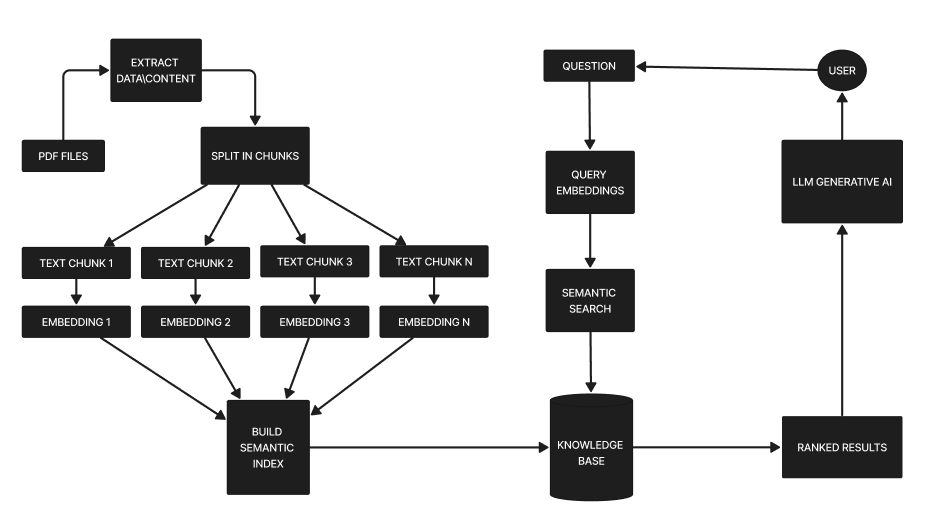
\includegraphics[width=\textwidth]{FLOWC}
    \caption{Proposed flowchart for P-BOT}
    \label{fig:your_image_label}
\end{figure*}

\subsection{Processing of Data}

The extraction of raw text from PDFs necessitates careful processing for effective storage and semantic search. An integral component of this process involves text chunking, a technique used to divide large text segments into smaller, more manageable units. Our examination highlights the impact of various chunking methods, including the NLTK Sentence Tokenizer, Spacy Sentence Splitter, and Langchain Character Text Splitter. Comparative analysis reveals that NLTK and Spacy consistently produce smaller, more digestible sentence segments, whereas Langchain generates larger and denser clusters of text.

Following the chunking process, the text segments are transformed into vector embeddings, numerical representations that capture word and sentence relationships. These embeddings are paramount for efficient storage and to improve semantic searches. By clustering related data points, they streamline the search process. Additionally, we investigate two distinct methods for generating these embeddings: OpenAI embeddings and Instructor embeddings. While OpenAI embeddings are known for their speed and accessibility via APIs, they come at a cost. In contrast, Instructor embeddings offer a budget-friendly alternative but exhibit slightly slower processing times.

\subsection{Storage of Data}

These embeddings are meticulously stored within specialized data repositories, commonly referred to as vector data stores. The vector data store is instrumental in streamlining the organization and retrieval of related data points, endowing LLMs with the capability to swiftly access and retrieve information. Several advanced technologies have emerged to facilitate the creation and utilization of vector data stores, including Facebook AI Similarity Search (FAISS), Pinecone, and Chroma. 

\subsection{Selection of Large language model}
We must choose a large language model capable of conducting query processing and semantic search within our vector datastore. To meet this requirement, we need a model that excels in natural language understanding, possesses context-awareness, and can generate pertinent responses or search results. Failure to satisfy these criteria could result in inaccurate, irrelevant, or misinterpreted query outcomes. Our research has identified several models that meet these requirements.

One of the most promising candidates is OpenAI's GPT-4, part of the GPT model family. It stands out as a versatile language model because can be customized for particular tasks through fine-tuning, including query processing and semantic search. This adaptability makes it a valuable asset for applications such as search engines and chatbots. Another strong contender is RoBERTa, short for Robustly Optimized BERT Approach. As an enhanced iteration of the BERT model, RoBERTa excels in comprehending and generating human language text. Its bidirectional approach, considering both left and right context, enhances its capability to grasp the intricate relationships between words in queries and documents, making it a valuable resource for our task

\subsection{Query Processing}
Once a user query is accepted, it undergoes a series of processing steps before our expansive language model can generate a response. The objective is to transform the query into a format that closely resembles the data stored within our vector data store. Initially, the query is divided into smaller units, like words or subword segments, through tokenization, referred to as tokens. These tokens are more manageable and amenable to further processing. Subsequently, these tokens are transformed into vector embeddings, using the same method we used for  converting data from our PDF documents into embeddings.

Upon completing this transformation, the query is prepared for processing by the large language model. These models are constructed based on the transformer architecture, which excels in managing sequential data, such as the text of the query. The transformer design encompasses numerous layers that employ self-attention and feedforward networks. This configuration enables the model to efficiently capture intricate relationships embedded within the input text. The query, in its embedded form, progresses through the neural network in a forward pass, with each layer meticulously analyzing the query. This enables the model to grasp crucial context and establish relationships among tokens. The outcome is a precise interpretation of the query by the model, resulting in more accurate and context-aware responses.

\subsection{Searching and Generation of response}
At the core of this operation resides the vector database, where data undergoes a transformation into vector embeddings, encapsulating the latent semantic content. Each document or informational entity is densely linked with a vector representation, thereby facilitating expedient searches rooted in semantic similarity. The evaluation of this similarity can be determined using cosine similarity, a mathematical metric renowned for assessing the resemblance between two non-zero vectors within the expansive terrain of high-dimensional space.

Following this critical step, the large language model commences the semantic search phase, leveraging its comprehension of the user's query to systematically search the vector database for documents or information that are semantically related. Those distinguished by the most elevated similarity scores are accorded the status of utmost relevance.

After collecting these pertinent documents or informational insights, the language model proceeds to the final phase: the generation of responses. The generated response is contextually relevant to the user's query and can take various forms, depending on the application—ranging from concise answers to a list of pertinent documents or even detailed explanations.



\section{Conclusion}
In conclusion, P-Bot stands as a revolutionary PDF chatbot, offering users the capability to effortlessly upload multiple or extensive PDFs and receive concise, summarized answers to their queries. Its advanced functionality not only streamlines information retrieval from voluminous documents but also enhances user convenience. P-Bot represents a significant leap forward in the realm of chatbot technology, providing a practical solution for efficiently extracting key insights from large sets of PDFs, ultimately empowering users in their information-seeking endeavors.

%\section{Ease of Use}
%\subsection{Selecting a Template}
%This template has been tailored for output on the custom paper size (8.26 cm x 11.22 cm). The margins are set as follows: top = 0.98 mm, bottom = 1.18 mm, right = 0.79 mm, left = 0.79 mm, space between column = 0.3 mm. The paragraphs must be indented. All paragraphs must be left justified and right justified.

%\subsection{Maintaining the Integrity of the Specifications} 
%The template is used to format your paper and style the text. All margins, column widths, line spaces, and text fonts are prescribed; please do not alter them. Your paper is one part of the entire proceedings, not an independent document. Please do not revise any of the current designations.

%Text font. The entire document should be in times New Roman font size 10. Paper title must be Left size, bold, regular font size 18 and the first letter of each word capitalized. Author names must be regular font size 10, bold. Author affiliation must be regular font size 9. Email addresses font size 9. Level 1 main headings must be Left size, bold, regular font size 12 and first word capitalized. Level 2 Sub headings must be left-justified, bold, italic, font size 11 and the first letter of each word capitalized.

%\section{Prepare Your Paper Before Styling}
%Before you begin to format your paper, first write and save the content as a separate text file. Keep your text and graphic files separate until after the text has been formatted and styled. Do not use hard tabs, and limit use of hard returns to only one return at the end of a paragraph. Do not add any kind of pagination anywhere in the paper. Do not number text heads-the template will do that for you.

%\subsection{Abbreviations and Acronyms} 
%Define abbreviations and acronyms the first time they are used in the text, even after they have been defined in the abstract. Do not use abbreviations in the title or headings unless they are unavoidable.

%\subsection{Units} 
%Use SI as primary units. English units may be used as secondary units (in parentheses). Use a zero before decimal points: “0.25”, not “.25”. Use “cm3”, not “cc”.

%\subsection{Equations} 
%The equations are an exception to the prescribed specifications of this template. You will need to determine whether or not your equation should be typed using either the Times New Roman or the Symbol font, Equations font size should be 9 and italic (please no other font). Equations should be edited by Math type, not in text or graphic versions. Number equations consecutively. Equation numbers, within parentheses, are to position flush right, as in (1), using a right tab stop.
%\linebreak

%Where:
%\begin{itemize}
%\item MC is the moisture content (\%)
%\item M1 is the initial weight of the wet sample (g)
%\item M2 is the weight of the dried sample (g)
%\end{itemize}

%Be sure that the symbols in your equation have been defined immediately following the equation. Use “Eq. 1”, not “Eq. (1)” or “Equation (1)”, and at the beginning of a sentence.

%\section{Using the Template}
%After the text edit has been completed, the paper is ready for the template. Duplicate the template file by using the Save As command. In this newly created file, highlight all of the contents and import your prepared text file. You are now ready to style your paper.

%\subsection{Authors and Affiliations} 
%The template is designed so that author affiliations are not repeated each time for multiple authors of the same affiliation. Please keep your affiliations as succinct as possible (do NOT post your job titles, positions, academic degrees, zip codes, names of building, street, district, province, state, etc.). This template was designed for two affiliations. You can adjust the template for authors with one affiliation or more than two affiliations.


%\subsection{Identify the Headings} 
%Sometimes mobile app Headings are organizational devices that guide the reader through your paper. There are two types: component headings and text heads. Component headings identify the different components of your paper and are not subordinate to each other. Examples include Introduction, Acknowledgments and References. Text heading organize the topics on a relational, hierarchical basis. If there are two or more sub-topics, the next level head should be used if there are not at least two sub-topics, then no subheads should be introduced.

%\begin{figure*}[ht]\centering % Using \begin{figure*} makes the figure take up the entire width of the page
%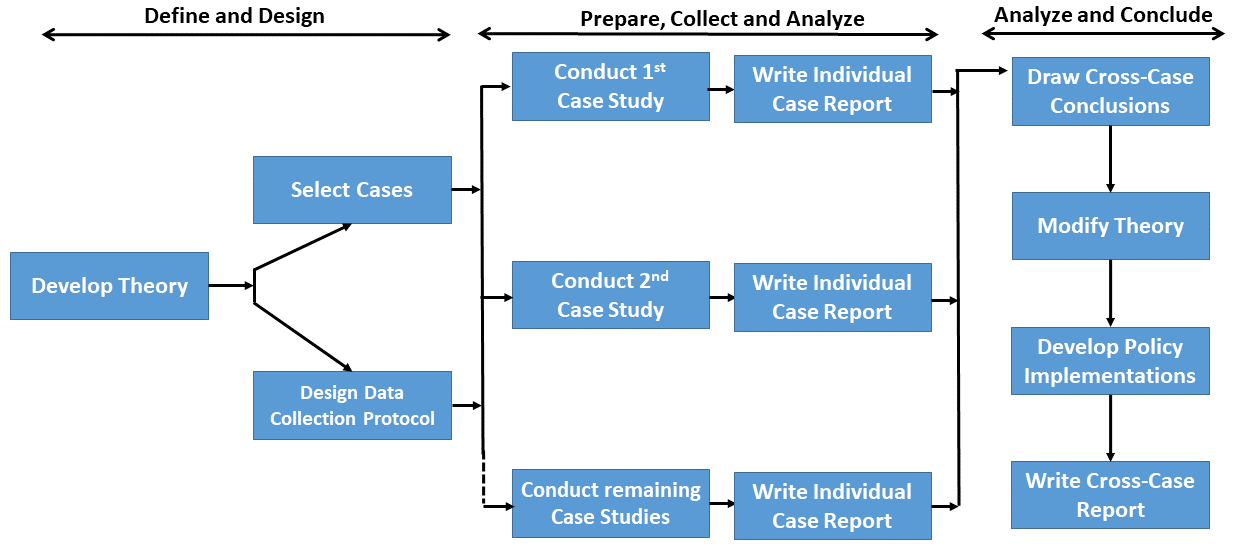
\includegraphics[width=\linewidth]{Multiple_case-study_design}
%\caption{Multiple Case Study Design \citep{yin2013case}}
%\label{Fig.Multiple_case-study_design}
%\end{figure*}

%\begin{table*}[!hbt]
%\caption{Demographics of four cases}
%\centering
%\begin{tabular}{ p{3cm}  p{3cm} p{3cm} p{3cm} p{3cm} }
%\toprule
%Case ID &   C1	&	C2	&	C3	&	C4 \\
%\midrule
%Business type & Software house & Software house & Software house & Software house \\
%Software house & National & International & International & National\\
%Dev. Method & Scrum Agile & Kanban Agile & Scrum Agile & Scrum Agile \\
%Mobile apps types & Games apps, Taxi apps & Business apps & Social apps, business apps & Hotel apps, travel apps\\
%Single user/ Enterprise apps & Single user& Enterprise & Enterprise&Single user \\
%Team size& 2 teams, each 5 members & 4 teams, each has 4 members & 5 teams, each has 5 members & 2 teams, each has 4 members\\
%\bottomrule
%\end{tabular}
%\label{table:demographics_info}
%\end{table*}

%\subsection{Figures and Tables} 
%Place figures and tables at the top or bottom of columns. Avoid placing them in the middle of columns. Large figures and tables may span across both columns. Figure captions should be below the figures; table heads should appear above the tables. Insert figures and tables after they are cited in the text. Use “Fig. 1” and “Table 1” even at the beginning of a sentence.

%Use Times New Roman font size 9 for Figure and Table labels. Use words rather than symbols or abbreviations when writing Figure axis labels to avoid confusing the reader. If include-ing units in the label, present them within parentheses. Label axes only with units just “A/m”. Do not label axes with a ratio of quantities and units. Graphs may be full color. Use only SOLID FILL COLORS which contrast well both on screen and hardcopy as shown in Fig. 1. When using photographs make sure the resolution is adequate to reveal important details as shown in Fig. 2.

%\section{Conclusion}
%The main conclusions of the experimental work should be presented. The contribution of the work to the scientific community and its economic implications should be emphasized.

%\section{Acknowledgement}
%Use same font size for the content of acknowledgements section.

%\section{Funding Information}
%The authors should acknowledge the funders of this manuscript and provide all necessary funding information.

%\section{Author’s Contributions}
%This section should state the contributions made by each author in the preparation, development and publication of this manuscript.

%\section{Ethics}
%Authors should address any ethical issues that may arise after the publication of this manuscript.


\section{References}
%Use the author/date system of references. In the text refer to the authors’ name (without initials) and year of publication. All publications cited in the text should be presented in a list of references following the text of the manuscript.

%\begin{enumerate}
%\item \subsection{Examples for a single author}
%Peterson (1993) has shown that...This is in agreement with the results obtained by several authors (Kramer, 1994; Smith, 1995; Brown, 1999)
%\item \subsection{Examples for two authors}
%Smith and White (1999) reported that....This was later found to be incorrect (Amir and Ahmed, 2000).

%\item \subsection{Examples for three or more authors}
%Moore et al. (1990) stated that...Similar results were reported recently (Smith et al., 2003).
%\end{enumerate}

\begin{enumerate}
\item \subsection{Journal Papers}
Wu, J., Gan, W., Chen, Z., Wan, S., and Lin, H. (2023). "AI-generated content (AIGC): A survey," arXiv preprint arXiv:2304.06632, pp. 1–17.

Wang, Y., Pan, Y., Yan, M., Su, Z., and Luan, T. H. (2023). "A Survey on ChatGPT: AI-Generated Contents, Challenges, and Solutions." arXiv preprint arXiv:2305.18339.

Wu, T., He, S., Liu, J., Sun, S., Liu, K., Han, Q.L., and Tang, Y. (2023). "A brief overview of ChatGPT: The history, status quo, and potential future development." IEEE/CAA Journal of Automatica Sinica, 10(5), pp. 1122-1136.

Gozalo-Brizuela, Roberto, and Eduardo C. Garrido-Merchan. "ChatGPT is not all you need. A State of the Art Review of large Generative AI models." arXiv preprint arXiv:2301.04655, 2023.

Mori, Shunji, Ching Y. Suen, and Kazuhiko Yamamoto. "Historical review of OCR research and development." Proceedings of the IEEE 80.7 (1992): 1029-1058.

Smith, Ray. "An overview of the Tesseract OCR engine." Ninth international conference on document analysis and recognition (ICDAR 2007). Vol. 2. IEEE, 2007.

Rabiner, L., and Juang, B. (1986). "An introduction to hidden Markov models." IEEE ASSP Magazine, 3(1), 4-16.

Mohd Yusoff, M. I., Mohamed, I., and Abu Bakar, M. R. (2014). "Hidden Markov models: An insight." Proceedings of the 6th International Conference on Information Technology and Multimedia, 259-264.

Viroli, C., and McLachlan, G. J. (2017). "Deep Gaussian mixture models." Statistics and Computing. doi:10.1007/s11222-017-9793-z

Pauls, Adam, and Dan Klein. "Faster and smaller n-gram language models." Proceedings of the 49th annual meeting of the Association for Computational Linguistics: Human Language Technologies. 2011.

Niesler, T. R., Woodland, P. C. (1996, May). A variable-length category-based n-gram language model. In 1996 IEEE International Conference on Acoustics, Speech, and Signal Processing Conference Proceedings (Vol. 1, pp. 164-167). IEEE.

Bickel, S., Haider, P.,  Scheffer, T. (2005, October). Predicting sentences using n-gram language models. In Proceedings of human language technology conference and conference on empirical methods in natural language processing (pp. 193-200).

Guthrie, D., Allison, B., Liu, W., Guthrie, L., and Wilks, Y. (2006, May). A closer look at skip-gram modelling. In LREC (Vol. 6, pp. 1222-1225).

Yin, Wenpeng, Ching Y. Suen, and Kazuhiko Yamamoto. "Comparative study of CNN and RNN for natural language processing." arXiv preprint arXiv:1702.01923 (2017).

Hochreiter, Sepp, and Jürgen Schmidhuber. "Long short-term memory." Neural computation 9.8 (1997): 1735-1780.

Hochreiter, Sepp. "The vanishing gradient problem during learning recurrent neural nets and problem solutions." International Journal of Uncertainty, Fuzziness and Knowledge-Based Systems 6.02 (1998): 107-116.

Liang, Zhiyao, and Shiru Zhang. "Generating and measuring similar sentences using long short-term memory and generative adversarial networks." IEEE Access 9 (2021): 112637-112654.

Miller, George A. "WordNet: a lexical database for English." Communications of the ACM 38.11 (1995): 39-41.

Wang, Kunfeng, et al. "Generative adversarial networks: introduction and outlook." IEEE/CAA Journal of Automatica Sinica 4.4 (2017): 588-598.

Tang, Xianlun, et al. "A multi-scale convolutional attention based GRU network for text classification." 2019 Chinese Automation Congress (CAC). IEEE, 2019.

Vaswani, Ashish, et al. "Attention is all you need." Advances in neural information processing systems 30 (2017).

Sarzynska-Wawer, Justyna, et al. "Detecting formal thought disorder by deep contextualized word representations." Psychiatry Research 304 (2021): 114135.

Kenton, Jacob Devlin Ming-Wei Chang, and Lee Kristina Toutanova. "Bert: Pre-training of deep bidirectional transformers for language understanding." Proceedings of naacL-HLT. Vol. 1. 2019.

Chen, Yiren, et al. "Improving bert with self-supervised attention." IEEE Access 9 (2021): 144129-144139.

Liu, Zhuang, et al. "A robustly optimized BERT pre-training approach with post-training." China National Conference on Chinese Computational Linguistics. Cham: Springer International Publishing, 2021.

Lewis, Mike, et al. "Bart: Denoising sequence-to-sequence pre-training for natural language generation, translation, and comprehension." arXiv preprint arXiv:1910.13461 (2019).

Radford, Alec, Karthik Narasimhan, Tim Salimans, and Ilya Sutskever. "Improving language understanding by generative pre-training." (2018).

Khosla, M., Anand, A., and  Setty, V. (2019). "A comprehensive comparison of unsupervised network representation learning methods." arXiv preprint arXiv:1903.07902.

Ieracitano, C., Paviglianiti, A., Campolo, M., Hussain, A., Pasero, E., and Morabito, F. C. (2021). "A novel automatic classification system based on hybrid unsupervised and supervised machine learning for electrospun nanofibers." IEEE/CAA J. Autom. Sinica, 8(1), 64–76.

Zong, Mingyu, and Bhaskar Krishnamachari. "A survey on GPT-3." arXiv preprint arXiv:2212.00857 (2022).

Radford, A., Wu, J., Child, R., Luan, D., Amodei, D. and Sutskever, I. (2019). "Language models are unsupervised multitask learners." OpenAI blog, 1(8), p.9.

Zhang, Y., and Yang, Q. (2022). "A survey on multi-task learning." IEEE Trans. Knowl. Data Eng., vol.34, no.12, pp.5586–5609.

Wang, Y. Q., Yao, Q. M., J. T. Kwok, and L. M. Ni. (2021). "Generalizing from a few examples: A survey on few-shot learning." ACM Comput. Surv., vol.53, no. 3, p. 63.

Khosla, M., A. Anand, and V. Setty. (2019). "A comprehensive comparison of unsupervised network representation learning methods." arXiv preprint arXiv: 1903.07902.

T. B. Brown, B. Mann, N. Ryder, M. Subbiah, J. Kaplan, P. Dhariwal, A. Neelakantan, P. Shyam, G. Sastry, A. Askell, S. Agarwal, A. Herbert-Voss, G. Krueger, T. Henighan, R. Child, A. Ramesh, D. M. Ziegler, J. Wu, C. Winter, C. Hesse, M. Chen, E. Sigler, M. Litwin, S. Gray, B. Chess, J. Clark, C. Berner, S. McCandlish, A. Radford, I. Sutskever, and D. Amodei. (2020). "Language models are few-shot learners." in Proc. 34th Int. Conf. Neural Information Processing Systems, Vancouver, Canada, pp. 1877–1901.

C. Finn, P. Abbeel, and S. Levine. (2017). "Model-agnostic meta-learning for fast adaptation of deep networks." in Proc. 34th Int. Conf. Machine Learning, Sydney, Australia, pp. 1126–1135.

J. Beck, R. Vuorio, E. Z. Liu, Z. Xiong, L. Zintgraf, C. Finn, and S. Whiteson. (2023). "A survey of meta-reinforcement learning." arXiv preprint arXiv: 2301.08028.

Q. X. Dong, L. Li, D. M. Dai, C. Zheng, Z. Y. Wu, B. B. Chang, X. Sun, J. J. Xu, L. Li, and Z. F. Sui. (2022). "A survey on in-context learning." arXiv preprint arXiv: 2301.00234.

L. Ouyang, J. Wu, X. Jiang, D. Almeida, C. L. Wainwright, P. Mishkin, C. Zhang, S. Agarwal, K. Slama, A. Ray, J. Schulman, J. Hilton, F. Kelton, L. Miller, M. Simens, A. Askell, P. Welinder, P. Christiano, J. Leike, and R. Lowe. (2022). "Training language models to follow instructions with human feedback." arXiv preprint arXiv: 2203.02155.

Ye, Junjie, et al. (2023). "A comprehensive capability analysis of gpt-3 and gpt-3.5 series models." arXiv preprint arXiv:2303.10420.




%\item \subsection{Text Book}
%Navabi, Z., 1998. Analysis and Modeling of Digital Systems.2nd Ed. McGraw Hill, New York. ISBN: 0070464790, pp: 632.
%\item \subsection{Book Chapter} Katz, R.H., 1986. Computer-Aided Design Databases. In: New Directions for Database Systems, Ariav, G. and J. Clifford, (Eds.), Intellect Books, Norwood, NJ, pp: 110-123. ISBN: 0893913448.
%\item \subsection{Conference Proceedings} Magott, J. and K. Skudlarski, 1989. Combining Generalized Stochastic Petri Nets and PERT Networks For The Performance Evaluation Of Concurrent Processes. Proceedings of the 3rd International Workshop on Petri Nets and Performance Models, Dec. 11-13, IEEE Xplore Press, Japan, pp: 249-256. DOI: 10.1109/PNPM.1989.68558.
%\item \subsection{Government Publications} United Nations, 2001. Indicators of Sustainable Development: Guidelines and Methodologies. United Nations Press, New York, USA.
\item \subsection{Online Publications} OpenAI. (2023). "Gpt-4 technical report." Available: https://cdn.openai.com/papers/gpt-4.pdf.

%\item \subsection{Generic Website}
%UNEP, 2002.Cleaner Production Assessment in Industries.Production and Consumption Branch. United Nations Environment Program. {URL} (Accessed on February 13, 2011)
%\item \subsection{Theses}
%Alkoaik, F., 2005. Fate of plant pathogens and pesticides during composting of greenhouse tomato plant residues. Unpublished dissertation in partial fulfillment of the requirements for the degree of Doctor of Philosophy, Dalhousie University, Halifax, Nova Scotia, Canada
\end{enumerate}

%-------------------------------------------------------------------------
%	REFERENCE LIST
%----------------------------------------------------------------------------------------
%\phantomsection
%\setlength{\bibsep}{0.5pt} % remove spaces between references
%\bibliographystyle{apalike} 
%\bibliography{references}
%\phantomsection

%----------------------------------------------------------------------------------------

\end{document}